\documentclass{beamer} 
\usepackage{amsmath,amsthm}
\usepackage{mathrsfs}
\usepackage{amssymb}
\usepackage[english]{babel}
\usepackage{latexsym}
\usepackage{amsfonts}
\usepackage{graphicx}
\usepackage{float}
\usepackage{graphics}
\usepackage{epsfig}
\usepackage{url}
\usepackage{soul}
\usepackage{listings}
\usepackage{bm}

% \usepackage{minted}


\usetheme{WVU}
\usecolortheme{WVU}
\usepackage{multirow}

\mode<presentation> 

\title[VE401 SU2022 RC week6]{VE401 SU2022 RC week6}

\author[ Shuyu Wu ]{ Shuyu Wu }
\institute[UM-SJTU JI]{UM-SJTU Joint Institute \vspace{.2cm} \\ 
\includegraphics[scale=0.3]{umji_logo.png}\\wushuyu2002@sjtu.edu.cn}
\date[June 2022]{\today}

\begin{document}
\begin{frame} 

\titlepage 

\end{frame} 
\section{Interval Estimation} 
\begin{frame}
       \frametitle{Outline}
       \tableofcontents[currentsection]
\end{frame}

\begin{frame}
    \frametitle{Problem of Point Estimation}
    In point estimation, we don't know how our estimation are close to the actual parameter.

\end{frame}

\begin{frame}
    \frametitle{Estimating the expectation of Normal Distribution}
    We have already known that when $X\sim N(\mu, \sigma^2)$, and $X_1, X_2, \dots , X_n$ are n i.i.d sample of $X$, then $\overline{X}$, as a random variable, $\overline{X}\sim N(\mu, \frac{\sigma^2}{n})$.\par
    Also we know $\overline{X}$ is an unbiased estimator of $\mu$. We know that 
    \[P[-a\leq \frac{\overline{X}-\mu}{\frac{\sigma}{\sqrt{n}}}\leq a]=\Phi(a)-\Phi(-a)=2\Phi(a)-1\]
    We hope this probability is determined, for example, 0.95, so when
    \[\Phi(a)=0.975\]
    The probability that $-a\frac{\sigma}{\sqrt{n}}\leq \mu \leq a\frac{\sigma}{\sqrt{n}}$ is 0.95


\end{frame}

\begin{frame}
    \frametitle{Upper Quantile $z_{\alpha}$}
    This notation will accompany you to the end of this course.\par
    We define $z_{\alpha}$ to be the inverse function of reliability function(survival function, $\alpha=1-\Phi(x)$). Or we can say that
    \[\alpha=P[Z>z_\alpha]\]
    This figure on slide 342 illustrate the relationship very well.
    \begin{figure}[H]
        \centering
        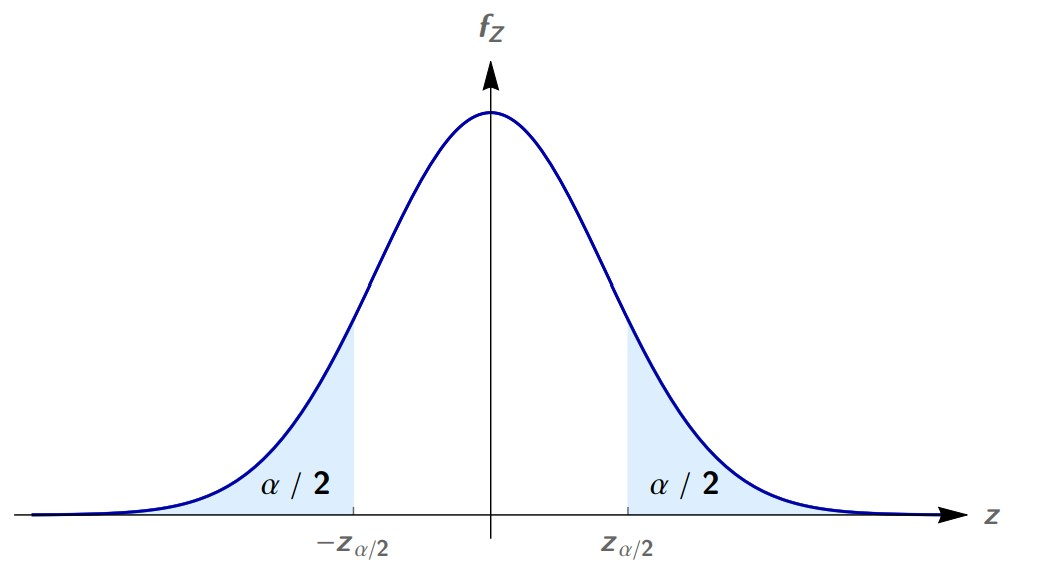
\includegraphics[width=0.37\textwidth,height=0.17\textwidth]{z_value.jpg}
        \caption{Interpretation of z-value}
    \end{figure}\par
    In python, you can get the value by function \href{https://docs.scipy.org/doc/scipy/reference/generated/scipy.stats.norm.html}{scipy.stats.norm.isf()}
    
\end{frame}

\begin{frame}
    \frametitle{Confidence Interval}

    So, $a=z_{0.025}$, thus we find that
    \[P[\mu\in [\overline{X} -z_{0.025} \frac{\sigma}{\sqrt{n}},\overline{X}+ z_{0.025} \frac{\sigma}{\sqrt{n}}]]=0.95\]
    This is called a 95\% confidence interval of $\mu$.\par

    Similarly, a $100(1-\alpha)\%$ (two-side) confidence interval for $\mu$ is given by
    \[[\overline{X} -z_{\alpha/2} \frac{\sigma}{\sqrt{n}},\overline{X}+ z_{\alpha/2} \frac{\sigma}{\sqrt{n}}]\]
    Or written down as
    \[\overline{X}\pm\frac{z_{\alpha/2}\cdot\sigma}{\sqrt{n}}\]

\end{frame}

\begin{frame}
    \frametitle{Confidence Interval}
    \textbf{Definition(two-sided):} let $\alpha\in[0,1]$, a $100(1-\alpha)\%$ two-sided confidence interval for a parameter $\theta$ is an interval $[L_1,L_2]$ such that $P[\theta\in[L_1,L_2]]=1-\alpha$.\par
    \textbf{Definition(one-sided):} let $\alpha\in[0,1]$, a $100(1-\alpha)\%$ upper confidence bound for a parameter $\theta$ is a number L such that $P[\theta\leq L]=1-\alpha$ ; a $100(1-\alpha)\%$ lower confidence bound for a parameter $\theta$ is a number L such that $P[\theta\geq L]=1-\alpha$.\par
    When the variance of normal distribution $X$ is known (denoted as $\sigma$): \par
    A $100(1-\alpha)\%$ upper confidence bound on $\mu$ is $\overline{X}+\frac{z_{\alpha}\cdot\sigma}{\sqrt{n}}$

    A $100(1-\alpha)\%$ lower confidence bound on $\mu$ is $\overline{X}-\frac{z_{\alpha}\cdot\sigma}{\sqrt{n}}$

\end{frame}

\begin{frame}
    \frametitle{ex 6.1}
    Here's a set of data:\par
    102.92742697 108.03584081  95.08485808 111.78162178 101.56169537
  98.66462405  90.42237418  95.75827205  99.58385681 104.96707954
  97.02704929  94.76337592  93.75187545 109.43115017  96.08087937
 107.8668476   95.06656345 105.32356197  99.65343386 109.87390971
 102.20971897 107.81314848  92.86804657 103.87540594 107.07219353
 103.87013897  97.50861952 100.64186604  97.57517754 104.37899888
  94.20918464  97.46665498  96.65737349  96.50775134 105.42586996
  99.95108958 102.42218598  99.50494885 101.02246684 112.38195949\par
  And we know the variance of the population is 25. What's the 95\% two-side confidence interval for the mean of the population?

\end{frame}

\begin{frame}
    \frametitle{ex 6.1 answer}
    First, you need to replace `` '' with ``,''. Use CTRL-H.\par
    The sample mean is 101.0247274005. We know the two-side confidence interval is $\overline{X}\pm\frac{z_{\alpha/2}\cdot\sigma}{\sqrt{n}}$. Now $\overline{X}=101.0247$, $z_{0.025}=1.96$, n=40, $\sigma=5$, the confidence interval is 
    \[101.0247\pm 1.550\]

\end{frame}

\begin{frame}
    \frametitle{When Variance is Unknown}
    When the variance $\sigma^2$ of the normal distribution, we use sample variance $S^2$ to estimate $\sigma^2$.
    \[S^2:=\frac{1}{n-1}\sum\limits_{k=1}^{n}(X_k-\overline{X})^2\]
    And we also want to know the distribution of $S^2$ to get the confidence interval of $\sigma^2$.\par
    By Helmert Transformation we can get the following important conclusion:


\end{frame}
\begin{frame}
    \frametitle{Conclusion of Sample Mean and Variance}
    \begin{enumerate}
        \item $\overline{X}$ and $S^2$ are independent
        \item $\overline{X}\sim N(\mu, \frac{\sigma^2}{n})$
        \item $\frac{(n-1)S^2}{\sigma^2}\sim \chi^2_{n-1}$
    \end{enumerate}
    
\end{frame}

\begin{frame}
    \frametitle{Upper Quantile of $\chi^2$ Distribution}
    The definition of $\chi^2_{\alpha,n}$ is similar to $z_{\alpha}$. It's the inverse survival function of chi-squared distribution with freedom of n.\par
    When $X\sim \chi^2_{n}$,
    \[P[X>\chi^2_{\alpha,n}]=\alpha\]
    \begin{figure}[H]
        \centering
        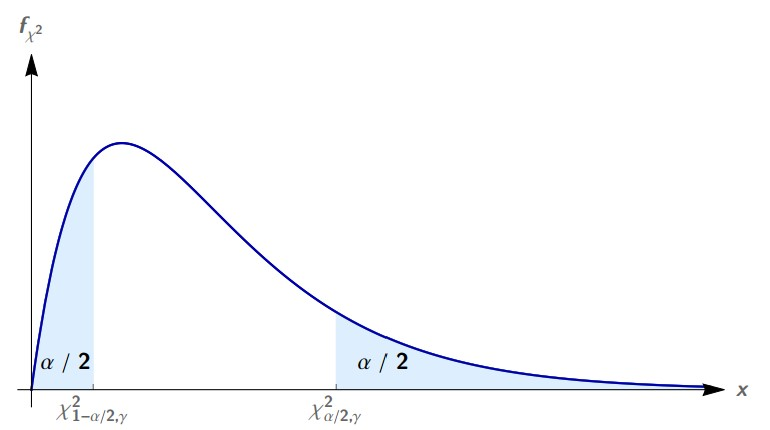
\includegraphics[width=0.42\textwidth,height=0.2\textwidth]{chi2val.jpg}
        \caption{Interpretation of chi2-value}
    \end{figure}\par
    From the figure above we can easily see that $P[\chi^2_{1-\alpha/2,n-1}\leq \frac{(n-1)S^2}{\sigma^2} \leq \chi^2_{\alpha/2,n-1}]=1-\alpha$\par
    In python, you can use the function \href{https://docs.scipy.org/doc/scipy/reference/generated/scipy.stats.chi2.html}{scipy.stats.chi2.isf()}

\end{frame}

\begin{frame}
    \frametitle{Confidence Interval of variance}
    The two-side confidence interval for $\sigma^2$ is
    \[[\frac{(n-1)S^2}{\chi_{\alpha/2,n-1}^2},\frac{(n-1)S^2}{\chi_{1-\alpha/2,n-1}^2}]\]
    A $100(1-\alpha)\%$ upper confidence interval for $\sigma^2$ is given by
    \[[0,\frac{(n-1)S^2}{\chi_{1-\alpha,n-1}^2}]\]
    A $100(1-\alpha)\%$ lower confidence interval for $\sigma^2$ is given by
    \[[\frac{(n-1)S^2}{\chi_{\alpha,n-1}^2},+\infty)\]
    

\end{frame}

\begin{frame}
    \frametitle{ex 6.2}
    Derive the 95\% \textbf{upper} confidence interval for the variance of the data. You don't know the overall variance(the data is the same in ex 6.1)
    

\end{frame}

\begin{frame}
    \frametitle{ex 6.2 answer}
    The sample variance is 30.933. $\chi^2_{0.95,40-1}=25.695$. The 95\% upper confidence interval is 
    \[[0,46.95]\]

\end{frame}

\begin{frame}
    \frametitle{Student T Distribution}
    A student T distribution with freedom $\gamma$ is defined as
    \[T_{\gamma}:=\frac{Z}{\sqrt{\chi^2_{\gamma}/\gamma}}\]
    When we don't know the overall variance $\sigma^2$, we have to use $S^2$. In this situation, $\frac{\overline{X}-\mu}{S/\sqrt{n}}$ is no longer a standard normal distribution. Instead, it's a T-distribution with freedom n-1.
    \[\frac{\overline{X}-\mu}{S/\sqrt{n}}=T_{n-1}\]

\end{frame}

\begin{frame}
    \frametitle{Confidence Interval for $\mu$ when $\sigma^2$ unknown}
    With $\sigma$ unknown, a $100(1-\alpha)\%$ two-sided confidence interval on $\mu$ is given by\[
    \overline{X}\pm\frac{t_{\alpha/2,n-1}\cdot S}{\sqrt{n}}\]

    $t_{\alpha,n}$ is the upper $\alpha$ quantile of $T_{n}$. In python, you can use the function with \href{https://docs.scipy.org/doc/scipy/reference/generated/scipy.stats.t.html}{scipy.stats.t.isf()}

    $\lim\limits_{n\to\infty}t_{\alpha,n}=z_{\alpha}$, and $t_{\alpha,n}>z_{\alpha}$
    

\end{frame}

\begin{frame}
    \frametitle{ex 6.3}

    Do the same thing for ex 6.1, except that you don't know the variance of the data.

\end{frame}

\begin{frame}
    \frametitle{ex 6.3 answer}

    $\overline{X}=101.0247, S^2=30.9333$, so $S=5.56$. $t_{0.025,39}=2.023$, so the 95\% two-side confidence interval for $\mu$ is 
    \[101.0247\pm 1.801\]

\end{frame}

\section{Extra topic and Q\&A}
\begin{frame}
    \frametitle{Outline}
    \tableofcontents[currentsection]
\end{frame}

\begin{frame}
    \frametitle{Extra topic}
    \begin{itemize}
        \item Practical tools
        \item How to quantitatively analysis whether a sample is normal distributed.
    \end{itemize}
    

\end{frame}


\begin{frame}
    \frametitle{Extra topic and Q\&A}
    
    Feel free to ask if you have any questions.\par
    The midterm exam is on 22nd, June. Topics include everything before interval estimation.
    
    
\end{frame}



\end{document} 